\documentclass{article}
\usepackage{amsthm,amsmath,amsfonts,lipsum}
\usepackage[T1]{fontenc}
\usepackage{beramono}
\usepackage{listings}
\usepackage{fontawesome5}
\usepackage{adjustbox}
\usepackage{mathabx}
\usepackage{thmtools}
\usepackage{import}
\usepackage{graphicx}
\usepackage{setspace}
\usepackage{geometry}
\usepackage{physics}
\usepackage{float}
\usepackage[english]{babel}
\usepackage{framed}
\usepackage[dvipsnames,x11names]{xcolor}
\usepackage{tcolorbox}
\usepackage{fancyhdr}
\usepackage{hyperref}
\usepackage{booktabs}
\usepackage{enumitem}
\usepackage{cancel}
\usepackage{background}
\usepackage{units}
\usepackage{mathtools}
\usepackage{bm}
\usepackage{caption}
\usepackage{esvect}

% Configuring the background
\backgroundsetup{
  scale=1, % Optional, scale if needed
  color=black, % Optional, set the image color, can be omitted
  opacity=0.18, % Optional, adjust opacity for watermark effect
  angle=0,
  position=current page.center, % Center the image on the page
  contents={
\includegraphics[width=1.75\paperwidth, height=1.75\paperheight, keepaspectratio]{ninym_ralei_leaf (watermarked by AlexanderTheMango)}} % Keeps aspect ratio and scales to fill the page
}

% Colours
\definecolor{darkgreen}{rgb}{0.0, 0.5, 0.0}
\definecolor{Firebrick}{rgb}{0.698, 0.132, 0.203}
\definecolor{Crimson}{rgb}{0.862745, 0.078431, 0.235294} % Crimson color
\definecolor{lightred}{rgb}{1.0, 0.819608, 0.819608} % Light red for background
\definecolor{MediumPurple}{rgb}{0.576, 0.439, 0.859}
\definecolor{chocolate}{rgb}{0.82, 0.41, 0.12} % Chocolate color definition
% Define the Navy color
\definecolor{Navy}{rgb}{0.0, 0.0, 0.5}

% Define custom tcolorbox styles for notes
\tcbuselibrary{skins, breakable}
\newtcolorbox{definitionbox}{colframe=RoyalBlue, colback=blue!5!white, title=Definition}
\newtcolorbox{examplebox}{colframe=ForestGreen, colback=green!5!white, title=Example}
\newtcolorbox{notebox}{colframe=RedOrange, colback=orange!5!white, title=Note}
\newtcolorbox{theorembox}{colframe=RoyalPurple, colback=purple!5!white, title=Theorem}

\newtcolorbox{propositionbox}{colframe=Goldenrod, colback=yellow!10!white, title=Proposition}
\newtcolorbox{remarkbox}{colframe=MidnightBlue, colback=blue!10!white, title=Remark}
\newtcolorbox{corollarybox}{colframe=OliveGreen, colback=green!10!white, title=Corollary}
\newtcolorbox{warningbox}{colframe=Crimson, colback=lightred, title=Warning}
\newtcolorbox{proofbox}{colframe=Black, colback=gray!10!white, title=Proof}
\newtcolorbox{questionbox}{colframe=Teal, colback=teal!10!white, title=Question}
\newtcolorbox{tipbox}{colframe=Goldenrod, colback=yellow!10!white, title=Tip}
\newtcolorbox{exercisebox}{colframe=darkgreen, colback=green!5!white, title=Exercise}
\newtcolorbox{solutionbox}{colframe=DodgerBlue4, colback=blue!5!white, title=Solution}
\newtcolorbox{algorithmbox}{colframe=Navy, colback=blue!10!white, title=Algorithm}
\newtcolorbox{conceptbox}{colframe=chocolate, colback=brown!10!white, title=Concept}
\newtcolorbox{illustrationbox}{colframe=Firebrick, colback=red!10!white, title=Illustration}
\newtcolorbox{intuitionbox}{colframe=MediumPurple, colback=purple!10!white, title=Intuition}
\newtcolorbox{answerbox}{colframe=RoyalBlue, colback=blue!10!white, title=Answer}

% Geometry settings
\geometry{letterpaper, portrait, includeheadfoot=true, hmargin=1in, vmargin=1in}
\onehalfspacing

% Header and footer
\pagestyle{fancy}
\fancyhf{}
\lhead{MAT232 - Lecture Notes}
\rhead{\thepage}
\lfoot{University of Toronto Mississauga}
\rfoot{\today}

% Document starts
\begin{document}
\renewcommand{\familydefault}{\rmdefault}

\begin{titlepage}
    \null % This is a TeX command that does nothing but is necessary for vfill to work correctly
    \vfill
    \begin{center}
        {\fontsize{40}{48}\selectfont \bfseries MAT232 - Lecture 13}
        \vspace{20pt} \\
        {\LARGE after partial derivatives?} \\
        \vspace{20pt}
        \textbf{AlexanderTheMango}
        \vspace{8pt}
        \\ Prepared for February 24, 2025
    \end{center}
    \vfill
\end{titlepage}

\addcontentsline{toc}{section}{Title Page}

\setcounter{page}{0}
\newpage
\tableofcontents
\newpage

\phantomsection
\begin{titlepage}
    \null % Ensures proper alignment with vfill
    \vfill
    \begin{center}
        {\Huge \textbf{Definitions and Theorems}} \\[20pt]
        \rule{\textwidth}{0.5mm} \\[15pt]
        {\Large \textit{Straight from the textbook — lots of fluff this time, more than what we need!}} \\[15pt]
        \rule{\textwidth}{0.5mm} \\[15pt]
        \textbf{Quick recap before diving into the lecture.}
    \end{center}
    \vfill
\end{titlepage}

\addcontentsline{toc}{section}{Preliminary Concepts}

\subsection*{Introduction to Vectors}
\addcontentsline{toc}{subsection}{Introduction to Vectors}

\begin{definitionbox}
    A \textbf{vector} is a quantity that has both magnitude and direction. Vectors can be optionally denoted in multiple ways:  

    \begin{itemize}
        \item \textbf{Boldface Notation}: \(\mathbf{v}\)  
        \item \textbf{Arrow Notation}: \(\vec{v}\)  
        \item \textbf{Overline Notation}: \(\overline{v}\)
    \end{itemize}  
    
    \begin{notebox}
    In MAT232H5, the contents of a vector are typically written using angle bracket notation:  
    
    \[
    \mathbf{v} = \langle v_1, v_2, v_3 \rangle
    \]
    
    For example, a 3D vector can be represented as:  
    
    \[
    \vec{v} = \langle 2, -1, 3 \rangle
    \]
    
    Depending on the context, you might see \(\mathbf{v} = \langle v_1, v_2 \rangle\) in 2D or \(\mathbf{v} = \langle v_1, v_2, v_3, v_4 \rangle\) in higher dimensions.
    \end{notebox}  
\end{definitionbox}

\begin{remarkbox} Quantities such as velocity and force are examples of vectors because they require both magnitude and direction to be fully described.
\end{remarkbox}

\subsection*{Vector Representation}
\addcontentsline{toc}{subsection}{Vector Representation}

A \textbf{vector} in a plane is represented by a directed line segment (an arrow) with an \textbf{initial point} and a \textbf{terminal point}. The length of the segment represents its \textbf{magnitude}, denoted \(\|\vec{v}\|\). A vector with the same initial and terminal point is called the \textbf{zero vector}, denoted \(\vec{0}\).  

\noindent
Two vectors \(\vec{v}\) and \(\vec{w}\) are \textbf{equivalent} if they have the same magnitude and direction, written as \(\vec{v} = \vec{w}\).

\begin{exercisebox}
    \textbf{Sketching Vectors} \\
    Sketch a vector in the plane from initial point \(P(1, 1)\) to terminal point \(Q(8, 5)\).
\end{exercisebox}

\subsection*{Basic Vector Operations}
\addcontentsline{toc}{subsection}{Basic Vector Operations}

\subsubsection*{Scalar Multiplication}
\addcontentsline{toc}{subsubsection}{Scalar Multiplication}

Multiplying a vector \(\vec{v}\) by a scalar \(k\) results in a new vector \(k\vec{v}\) with the following properties:
\begin{itemize}[label=\labelitemiv, left=2pt]
    \item Its magnitude is \(|k|\) times the magnitude of \(\vec{v}\).  
    \item Its direction remains the same if \(k > 0\).  
    \item Its direction is reversed if \(k < 0\).  
    \item If \(k = 0\) or \(\vec{v} = \vec{0}\), then \(k\vec{v} = \vec{0}\).  
\end{itemize}
\begin{notebox}
The zero vector \(\vec{0}\) is the vector with a magnitude of 0 and no direction (or any direction). 
It is the only vector that is orthogonal (perpendicular) to every vector, including itself.
\end{notebox}

\begin{exercisebox}
    \textbf{Scalar Multiplication} \\
    Given vector \(\vv{v}\), sketch the vectors \(3\vv{v}\), \(\frac{1}{2}\vv{v}\), and \(-\vv{v}\).
\end{exercisebox}

\subsubsection*{Vector Addition}
\addcontentsline{toc}{subsubsection}{Vector Addition}

The sum of two vectors \(\vv{v}\) and \(\vv{w}\) is constructed by placing the initial point of \(\vv{w}\) at the terminal point of \(\vv{v}\). The vector sum, \(\vv{v} + \vv{w}\), is the vector from the initial point of \(\vv{v}\) to the terminal point of \(\vv{w}\).

\begin{exercisebox}
    \textbf{Vector Addition} \\
    Given vectors \(\vv{v}\) and \(\vv{w}\), sketch \(\vv{v} + \vv{w}\) using both the triangle method and the parallelogram method.
    \begin{figure}[H]
        \centering
        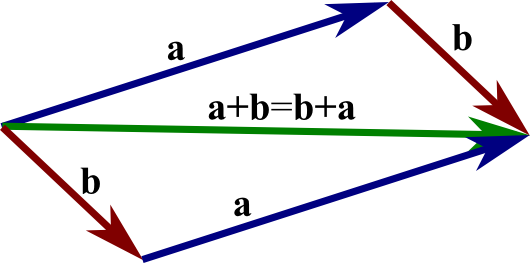
\includegraphics[width=0.55\textwidth]{add-vectors.png}
    \end{figure}
\end{exercisebox}

\subsubsection*{Vector Subtraction}
\addcontentsline{toc}{subsubsection}{Vector Subtraction}

The difference \(\vv{v} - \vv{w}\) is defined as \(\vv{v} + (-\vv{w})\), where \(-\vv{w}\) is the vector with the same magnitude as \(\vv{w}\) but opposite direction.

\begin{exercisebox}
    \textbf{Vector Subtraction} \\
    Given vectors \(\vv{v}\) and \(\vv{w}\), sketch \(\vv{v} - \vv{w}\).
\end{exercisebox}

\subsection*{Vector Components}
\addcontentsline{toc}{subsection}{Vector Components}

A vector in standard position has its initial point at the origin \((0, 0)\). If the terminal point is \((x, y)\), the vector is written in \textbf{component form} as \(\vv{v} = \langle x, y \rangle\). The scalars \(x\) and \(y\) are called the \textbf{components} of \(\vv{v}\).

\begin{exercisebox}
    \textbf{Expressing Vectors in Component Form} \\
    Express vector \(\vv{v}\) with initial point \((-3, 4)\) and terminal point \((1, 2)\) in component form.
\end{exercisebox}

\subsection*{Magnitude of a Vector}
\addcontentsline{toc}{subsection}{Magnitude of a Vector}

\begin{definitionbox}
    The magnitude of a vector \(\vv{v} = \langle x, y \rangle\) is its length, and is given by:
    \[
    \|\vv{v}\| = \sqrt{x^2 + y^2}.
    \]
\end{definitionbox}

\begin{exercisebox}
    Find the magnitude of the vector \(\vv{v} = \langle 3, -4 \rangle\).
\end{exercisebox}

\subsection*{Properties of Vector Operations}
\addcontentsline{toc}{subsection}{Properties of Vector Operations}

\begin{theorembox}
    Let \(\vv{u}\), \(\vv{v}\), and \(\vv{w}\) be vectors, and let \(k\) and \(c\) be scalars. Then:
    \begin{enumerate}
        \item \(\vv{u} + \vv{v} = \vv{v} + \vv{u}\) \quad (Commutative Property)
        \item \((\vv{u} + \vv{v}) + \vv{w} = \vv{u} + (\vv{v} + \vv{w})\) \quad (Associative Property)
        \item \(k(c\vv{v}) = (kc)\vv{v}\) \quad (Associativity of Scalar Multiplication)
        \item \(k(\vv{u} + \vv{v}) = k\vv{u} + k\vv{v}\) \quad (Distributive Property)
    \end{enumerate}
\end{theorembox}

\begin{proofbox}
    \textbf{Proof of Commutative Property:}
    \begin{proof}
    Let \(\vv{u} = \langle u_1, u_2 \rangle\) and \(\vv{v} = \langle v_1, v_2 \rangle\). Then:
    \[
    \vv{u} + \vv{v} = \langle u_1 + v_1, u_2 + v_2 \rangle = \langle v_1 + u_1, v_2 + u_2 \rangle = \vv{v} + \vv{u}.
    \]
    \end{proof}
\end{proofbox}

\subsection*{Applications of Vectors}
\addcontentsline{toc}{subsection}{Applications of Vectors}

\begin{examplebox}
    \textbf{Real-Life Applications}
    \begin{itemize}
        \item A boat crossing a river experiences a force from its motor and a force from the river current. Both forces are vectors.
        \item A quarterback throwing a football applies a velocity vector to the ball, determining its speed and direction.
    \end{itemize}
\end{examplebox}

\subsection*{Introduction to Three-Dimensional Space}
\addcontentsline{toc}{subsection}{Introduction to Three-Dimensional Space}

The \textbf{three-dimensional rectangular coordinate system} consists of three perpendicular axes: the \(x\)-axis, the \(y\)-axis, and the \(z\)-axis, with an origin at the point of intersection \((0, 0, 0)\). This system is often denoted by \(\mathbb{R}^3\).

\begin{tipbox}
    The three-dimensional coordinate system follows the \textbf{right-hand rule}. If you align your right hand’s fingers with the positive \(x\)-axis and curl them toward the positive \(y\)-axis, your thumb points in the direction of the positive \(z\)-axis.
    \begin{remarkbox}
        This can also be visualized by holding a screwdriver with your right hand. If you rotate the screwdriver from the positive \(x\)-axis to the positive \(y\)-axis, the direction of the screwdriver represents the positive \(z\)-axis.
    \end{remarkbox}
    \begin{notebox}
        The right-hand rule can serve as a visual aid for determining the direction of the cross product of two vectors.
    \end{notebox}
\end{tipbox}

\subsection*{Locating Points in Space}
\addcontentsline{toc}{subsection}{Locating Points in Space}

A point in three-dimensional space is represented by coordinates \((x, y, z)\), where:
\begin{itemize}
    \item \(x\) is the distance along the \(x\)-axis,
    \item \(y\) is the distance along the \(y\)-axis,
    \item \(z\) is the distance along the \(z\)-axis.
\end{itemize}

\begin{exercisebox}
    Sketch the points \((-2, 3, -1)\) and \((1, -2, 3)\) in three-dimensional space.
\end{exercisebox}

\subsection*{Coordinate Planes in \(\mathbb{R}^3\)}
\addcontentsline{toc}{subsection}{Coordinate Planes in \(\mathbb{R}^3\)}

The three coordinate planes in \(\mathbb{R}^3\) are:
\begin{itemize}
    \item The \(xy\)-plane: \(\{(x, y, 0) \mid x, y \in \mathbb{R}\}\),
    \item The \(xz\)-plane: \(\{(x, 0, z) \mid x, z \in \mathbb{R}\}\),
    \item The \(yz\)-plane: \(\{(0, y, z) \mid y, z \in \mathbb{R}\}\).
\end{itemize}

\begin{notebox}
    The coordinate planes divide space into eight regions called \textbf{octants}. The first octant is where \(x > 0\), \(y > 0\), and \(z > 0\); the other octants are numbered counterclockwise.
    It's like quadrants in 2D, but with that extra dimension!
\end{notebox}

\subsection*{Distance Formula in Three Dimensions}
\addcontentsline{toc}{subsection}{Distance Formula in Three Dimensions}

\begin{theorembox}
    The distance \(d\) between points \(P_1 = (x_1, y_1, z_1)\) and \(P_2 = (x_2, y_2, z_2)\) is given by:
    \[
    d = \sqrt{(x_2 - x_1)^2 + (y_2 - y_1)^2 + (z_2 - z_1)^2}.
    \]
\end{theorembox}

\begin{exercisebox}
    Find the distance between points \(P_1 = (1, -5, 4)\) and \(P_2 = (4, -1, -1)\).
\end{exercisebox}

\subsection*{Equations of Planes}
\addcontentsline{toc}{subsection}{Equations of Planes}

A plane parallel to one of the coordinate planes can be described by:
\begin{itemize}
    \item \(z = c\) for a plane parallel to the \(xy\)-plane,
    \item \(y = b\) for a plane parallel to the \(xz\)-plane,
    \item \(x = a\) for a plane parallel to the \(yz\)-plane.
\end{itemize}

\begin{exercisebox}
    Write an equation of the plane passing through point \((1, -6, -4)\) that is parallel to the \(xy\)-plane.
\end{exercisebox}

\subsection*{Equations of Spheres}
\addcontentsline{toc}{subsection}{Equations of Spheres}

\begin{definitionbox}
    A \textbf{sphere} is the shape described by the set of all points in space equidistant from a fixed point, called the \textbf{centre}. The distance from the centre to any point on the sphere is called the \textbf{radius}.
\end{definitionbox}

\begin{theorembox}
    \textbf{Equation of a Sphere:} \\
    The sphere with centre \((a, b, c)\) and radius \(r\) is given by:
    \[
    (x - a)^2 + (y - b)^2 + (z - c)^2 = r^2.
    \]
\end{theorembox}

\begin{exercisebox}
    Find the standard equation of the sphere with center \((-2, 4, -5)\) and passing through point \((4, 4, -1)\).
\end{exercisebox}

\begin{exercisebox}
    Find the equation of the sphere with diameter \(PQ\), where \(P = (2, -1, -3)\) and \(Q = (-2, 5, -1)\).
\end{exercisebox}

\subsection*{Example: Describing and Graphing a Set of Points}
\addcontentsline{toc}{subsection}{Example: Describing and Graphing a Set of Points}

\begin{examplebox}
    Describe and graph the set of points satisfying \((y + 2)(z - 3) = 0\).

    \begin{solutionbox}
        The equation implies \( y + 2 = 0 \) or \( z - 3 = 0 \), giving the solution set:
        \[
        y = -2 \quad \text{or} \quad z = 3.
        \]
        Geometrically, this represents two planes:
        \begin{itemize}
            \item \( y = -2 \): A plane parallel to the \( xz \)-plane.
            \item \( z = 3 \): A plane parallel to the \( xy \)-plane.
        \end{itemize}
        These planes intersect along the line \( y = -2, z = 3 \), parallel to the \( x \)-axis. The graph consists of these two planes meeting along this line.

        \begin{figure}[H]
            \centering
            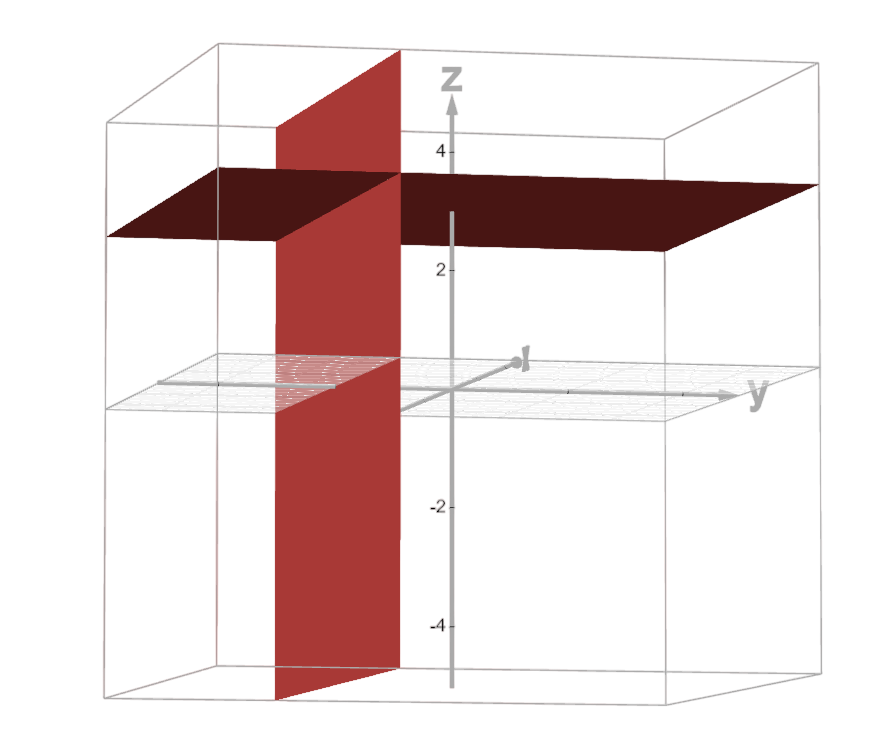
\includegraphics[width=0.6\textwidth]{(y+2)(z-3)=0.png}
            \caption{Graph of \( (y + 2)(z - 3) = 0 \), represented by two planes intersecting along the line where \(y = -2\) and \(z = 3\).}
            \label{fig:two_planes}
        \end{figure}
    \end{solutionbox}
\end{examplebox}

\begin{tipbox}
Graphing such equations involves visualizing the planes and their intersection in three-dimensional space.
\end{tipbox}

\begin{examplebox}
    Describe and graph the set of points satisfying \(x^2 + (z - 2)^2 = 16\).

    \begin{solutionbox}
        The given equation represents a \textbf{circular cylinder} in three-dimensional space:
        \[
        x^2 + (z - 2)^2 = 16.
        \]
        This describes a cylinder with:
        \begin{itemize}
            \item \textbf{Center:} \((0,2)\) in the \( xz \)-plane.
            \item \textbf{Radius:} \(4\).
            \item \textbf{Axis:} Parallel to the \( y \)-axis, meaning it extends infinitely along \( y \).
        \end{itemize}

        \textbf{Graphing:}
        \begin{itemize}
            \item Draw a circle of radius \(4\) centered at \( (0,2) \) in the \( xz \)-plane.
            \item Extend this shape infinitely in the \( y \)-direction to form the cylinder.
        \end{itemize}

        \begin{figure}[H]
            \centering
            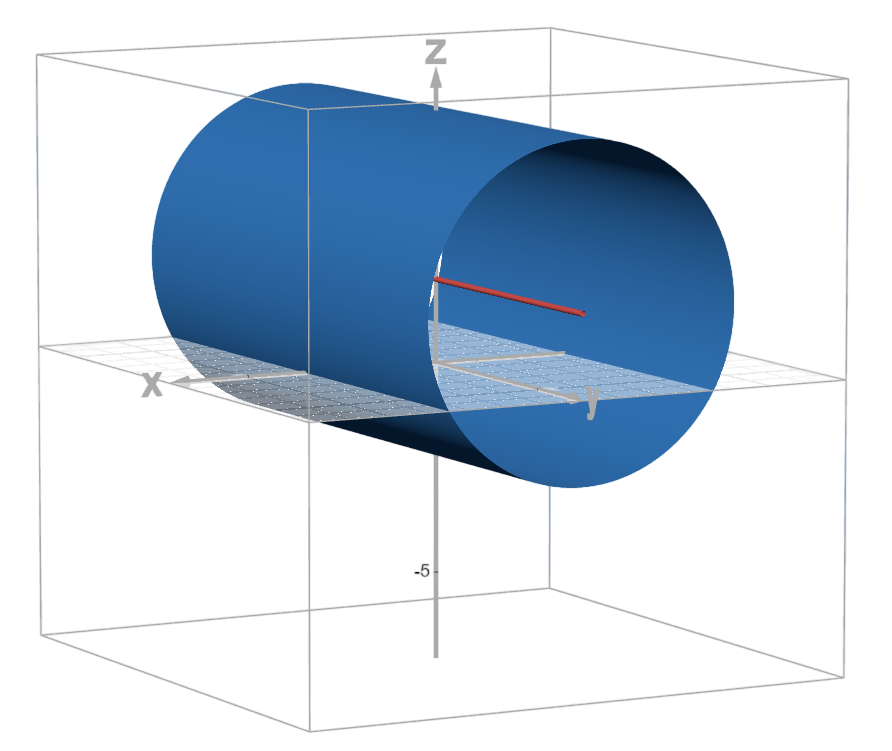
\includegraphics[width=0.6\textwidth]{x^2+(z-2)^2=16.png}
            \caption{Graph of \( x^2 + (z - 2)^2 = 16 \), representing a circular cylinder with center \((0,2)\) and radius \(4\).}
            \label{fig:circular_cylinder}
        \end{figure}
    \end{solutionbox}
\end{examplebox}

\subsection*{Working with Vectors in \(\mathbb{R}^3\)}
\addcontentsline{toc}{subsection}{Working with Vectors in \(\mathbb{R}^3\)}

\begin{definitionbox}
    A \textbf{three-dimensional vector} is a quantity with both magnitude and direction, represented by a directed line segment (arrow) in \(\mathbb{R}^3\). A vector \(\vv{v} = \langle x, y, z \rangle\) has its initial point at the origin \((0, 0, 0)\) and its terminal point at \((x, y, z)\). The zero vector is \(\vv{0} = \langle 0, 0, 0 \rangle\).
\end{definitionbox}

\begin{exercisebox}
    Let \(S = (3, 8, 2)\) and \(T = (2, -1, 3)\). Express \(\vv{ST}\) in component form and in standard unit form.
\end{exercisebox}

\subsection*{Vector Operations in \(\mathbb{R}^3\)}
\addcontentsline{toc}{subsection}{Vector Operations in \(\mathbb{R}^3\)}

\begin{definitionbox}
    Let \(\vv{v} = \langle x_1, y_1, z_1 \rangle\) and \(\vv{w} = \langle x_2, y_2, z_2 \rangle\) be vectors in \(\mathbb{R}^3\), and let \(k\) be a scalar. Then:
    \begin{itemize}
        \item \textbf{Vector Addition:} \(\vv{v} + \vv{w} = \langle x_1 + x_2, y_1 + y_2, z_1 + z_2 \rangle\)
        \item \textbf{Scalar Multiplication:} \(k\vv{v} = \langle kx_1, ky_1, kz_1 \rangle\)
        \item \textbf{Vector Subtraction:} \(\vv{v} - \vv{w} = \vv{v} + (-\vv{w}) = \langle x_1 - x_2, y_1 - y_2, z_1 - z_2 \rangle\)
        \item \textbf{Magnitude:} \(\|\vv{v}\| = \sqrt{x_1^2 + y_1^2 + z_1^2}\)
        \item \textbf{Unit Vector:} The unit vector in the direction of \(\vv{v}\) is \(\frac{1}{\|\vv{v}\|} \vv{v}\), provided \(\vv{v} \neq \vv{0}\).
    \end{itemize}
\end{definitionbox}

\begin{exercisebox}
    \textbf{Vector Operations in Three Dimensions} \\
    Let \(\vv{v} = \langle -2, 9, 5 \rangle\) and \(\vv{w} = \langle 1, -1, 0 \rangle\). Find the following vectors:
    \begin{itemize}
        \item \(3\vv{v} - 2\vv{w}\)
        \item \(5\|\vv{w}\|\)
        \item \(\|5\vv{w}\|\)
        \item A unit vector in the direction of \(\vv{v}\)
    \end{itemize}
\end{exercisebox}

\begin{exercisebox}
    Let \(\vv{v} = \langle -1, -1, 1 \rangle\) and \(\vv{w} = \langle 2, 0, 1 \rangle\). Find a unit vector in the direction of \(5\vv{v} + 3\vv{w}\).
\end{exercisebox}

\subsection*{Properties of Vectors in \(\mathbb{R}^3\)}
\addcontentsline{toc}{subsection}{Properties of Vectors in \(\mathbb{R}^3\)}

\begin{theorembox}
    \textbf{Properties of Vectors in Space:} \\
    Let \(\vv{u}\), \(\vv{v}\), and \(\vv{w}\) be vectors in \(\mathbb{R}^3\), and let \(k\) and \(c\) be scalars. Then:
    \begin{enumerate}
        \item \(\vv{u} + \vv{v} = \vv{v} + \vv{u}\) \quad (Commutative Property)
        \item \((\vv{u} + \vv{v}) + \vv{w} = \vv{u} + (\vv{v} + \vv{w})\) \quad (Associative Property)
        \item \(\vv{u} + \vv{0} = \vv{u}\) \quad (Additive Identity Property)
        \item \(\vv{u} + (-\vv{u}) = \vv{0}\) \quad (Additive Inverse Property)
        \item \(k(c\vv{v}) = (kc)\vv{v}\) \quad (Associativity of Scalar Multiplication)
        \item \(k(\vv{u} + \vv{v}) = k\vv{u} + k\vv{v}\) \quad (Distributive Property)
        \item \((k + c)\vv{u} = k\vv{u} + c\vv{u}\) \quad (Distributive Property)
        \item \(1\vv{u} = \vv{u}\) and \(0\vv{u} = \vv{0}\) \quad (Identity and Zero Properties)
    \end{enumerate}
\end{theorembox}

\begin{proofbox}
    \textbf{Proof of Commutative Property:}
    \begin{proof}
    Let \(\vv{u} = \langle u_1, u_2, u_3 \rangle\) and \(\vv{v} = \langle v_1, v_2, v_3 \rangle\). Then:
    \[
    \vv{u} + \vv{v} = \langle u_1 + v_1, u_2 + v_2, u_3 + v_3 \rangle = \langle v_1 + u_1, v_2 + u_2, v_3 + u_3 \rangle = \vv{v} + \vv{u}.
    \]
    \end{proof}
\end{proofbox}

\textbf{self-note: embellish the following}

\subsection*{The Dot Product and Its Properties}
\addcontentsline{toc}{subsection}{The Dot Product and Its Properties}

\begin{definitionbox}
    \textbf{Definition:} The \textbf{dot product} of vectors \(\vv{u} = \langle u_1, u_2, u_3 \rangle\) and \(\vv{v} = \langle v_1, v_2, v_3 \rangle\) is given by:
    \[
    \vv{u} \cdot \vv{v} = u_1 v_1 + u_2 v_2 + u_3 v_3.
    \]
    For two-dimensional vectors \(\vv{u} = \langle u_1, u_2 \rangle\) and \(\vv{v} = \langle v_1, v_2 \rangle\), the dot product is:
    \[
    \vv{u} \cdot \vv{v} = u_1 v_1 + u_2 v_2.
    \]
\end{definitionbox}

\begin{examplebox}
    \textbf{Example 2.21: Calculating Dot Products} \\
    \begin{itemize}
        \item Find the dot product of \(\vv{u} = \langle 3, 5, 2 \rangle\) and \(\vv{v} = \langle -1, 3, 0 \rangle\).
        \item Find the scalar product of \(\vv{p} = 10\vv{i} - 4\vv{j} + 7\vv{k}\) and \(\vv{q} = -2\vv{i} + \vv{j} + 6\vv{k}\).
    \end{itemize}
\end{examplebox}

\begin{exercisebox}
    \textbf{Checkpoint 2.21:} \\
    Find \(\vv{u} \cdot \vv{v}\), where \(\vv{u} = \langle 2, 9, -1 \rangle\) and \(\vv{v} = \langle -3, 1, -4 \rangle\).
\end{exercisebox}

\subsection*{Properties of the Dot Product}
\addcontentsline{toc}{subsection}{Properties of the Dot Product}

\begin{theorembox}
    \textbf{Theorem 2.3: Properties of the Dot Product} \\
    Let \(\vv{u}\), \(\vv{v}\), and \(\vv{w}\) be vectors, and let \(c\) be a scalar. Then:
    \begin{enumerate}
        \item \(\vv{u} \cdot \vv{v} = \vv{v} \cdot \vv{u}\) \quad (Commutative Property)
        \item \(\vv{u} \cdot (\vv{v} + \vv{w}) = \vv{u} \cdot \vv{v} + \vv{u} \cdot \vv{w}\) \quad (Distributive Property)
        \item \(c(\vv{u} \cdot \vv{v}) = (c\vv{u}) \cdot \vv{v} = \vv{u} \cdot (c\vv{v})\) \quad (Associative Property)
        \item \(\vv{v} \cdot \vv{v} = \|\vv{v}\|^2\) \quad (Property of Magnitude)
    \end{enumerate}
\end{theorembox}

\begin{proofbox}
    \textbf{Proof of Commutative Property:}
    \begin{proof}
    Let \(\vv{u} = \langle u_1, u_2, u_3 \rangle\) and \(\vv{v} = \langle v_1, v_2, v_3 \rangle\). Then:
    \[
    \vv{u} \cdot \vv{v} = u_1 v_1 + u_2 v_2 + u_3 v_3 = v_1 u_1 + v_2 u_2 + v_3 u_3 = \vv{v} \cdot \vv{u}.
    \]
    \end{proof}
\end{proofbox}

\begin{examplebox}
    \textbf{Example 2.22: Using Properties of the Dot Product} \\
    Let \(\vv{a} = \langle 1, 2, -3 \rangle\), \(\vv{b} = \langle 0, 2, 4 \rangle\), and \(\vv{c} = \langle 5, -1, 3 \rangle\). Find each of the following products:
    \begin{itemize}
        \item \((\vv{a} \cdot \vv{b}) \vv{c}\)
        \item \(\vv{a} \cdot (2\vv{c})\)
        \item \(\|\vv{b}\|^2\)
    \end{itemize}
\end{examplebox}

\begin{exercisebox}
    \textbf{Checkpoint 2.22:} \\
    Find the following products for \(\vv{p} = \langle 7, 0, 2 \rangle\), \(\vv{q} = \langle -2, 2, -2 \rangle\), and \(\vv{r} = \langle 0, 2, -3 \rangle\):
    \begin{itemize}
        \item \((\vv{r} \cdot \vv{p}) \vv{q}\)
        \item \(\|\vv{p}\|^2\)
    \end{itemize}
\end{exercisebox}

\subsection*{Using the Dot Product to Find the Angle Between Two Vectors}
\addcontentsline{toc}{subsection}{Using the Dot Product to Find the Angle Between Two Vectors}

\begin{theorembox}
    \textbf{Theorem 2.4: Evaluating a Dot Product} \\
    The dot product of two vectors is the product of the magnitude of each vector and the cosine of the angle between them:
    \[
    \vv{u} \cdot \vv{v} = \|\vv{u}\| \|\vv{v}\| \cos \theta.
    \]
\end{theorembox}

\begin{examplebox}
    \textbf{Example 2.23: Finding the Angle Between Two Vectors} \\
    Find the measure of the angle between each pair of vectors:
    \begin{itemize}
        \item \(\vv{i} + \vv{j} + \vv{k}\) and \(2\vv{i} - \vv{j} - 3\vv{k}\)
        \item \(\langle 2, 5, 6 \rangle\) and \(\langle -2, -4, 4 \rangle\)
    \end{itemize}
\end{examplebox}

\begin{exercisebox}
    \textbf{Checkpoint 2.23:} \\
    Find the measure of the angle, in radians, formed by vectors \(\vv{a} = \langle 1, 2, 0 \rangle\) and \(\vv{b} = \langle 2, 4, 1 \rangle\). Round to the nearest hundredth.
\end{exercisebox}

\subsection*{Orthogonal Vectors}
\addcontentsline{toc}{subsection}{Orthogonal Vectors}

\begin{theorembox}
    \textbf{Theorem 2.5: Orthogonal Vectors} \\
    The nonzero vectors \(\vv{u}\) and \(\vv{v}\) are orthogonal if and only if \(\vv{u} \cdot \vv{v} = 0\).
\end{theorembox}

\begin{examplebox}
    \textbf{Example 2.24: Identifying Orthogonal Vectors} \\
    Determine whether \(\vv{p} = \langle 1, 0, 5 \rangle\) and \(\vv{q} = \langle 10, 3, -2 \rangle\) are orthogonal vectors.
\end{examplebox}

\begin{exercisebox}
    \textbf{Checkpoint 2.24:} \\
    For which value of \(x\) is \(\vv{p} = \langle 2, 8, -1 \rangle\) orthogonal to \(\vv{q} = \langle x, -1, 2 \rangle\)?
\end{exercisebox}

\subsection*{Direction Cosines}
\addcontentsline{toc}{subsection}{Direction Cosines}

\begin{definitionbox}
    \textbf{Definition:} The \textbf{direction angles} of a nonzero vector \(\vv{v}\) are the angles \(\alpha\), \(\beta\), and \(\gamma\) that \(\vv{v}\) makes with the positive \(x\)-, \(y\)-, and \(z\)-axes, respectively. The cosines of these angles are called the \textbf{direction cosines}:
    \[
    \cos \alpha = \frac{v_1}{\|\vv{v}\|}, \quad \cos \beta = \frac{v_2}{\|\vv{v}\|}, \quad \cos \gamma = \frac{v_3}{\|\vv{v}\|}.
    \]
\end{definitionbox}

\begin{examplebox}
    \textbf{Example 2.25: Measuring the Angle Formed by Two Vectors} \\
    Let \(\vv{v} = \langle 2, 3, 3 \rangle\). Find the measures of the angles formed by:
    \begin{itemize}
        \item \(\vv{v}\) and \(\vv{i}\)
        \item \(\vv{v}\) and \(\vv{j}\)
        \item \(\vv{v}\) and \(\vv{k}\)
    \end{itemize}
\end{examplebox}

\begin{exercisebox}
    \textbf{Checkpoint 2.25:} \\
    Let \(\vv{v} = \langle 3, -5, 1 \rangle\). Find the measure of the angles formed by:
    \begin{itemize}
        \item \(\vv{v}\) and \(\vv{i}\)
        \item \(\vv{v}\) and \(\vv{j}\)
        \item \(\vv{v}\) and \(\vv{k}\)
    \end{itemize}
\end{exercisebox}

\subsection*{Vector Projections}
\addcontentsline{toc}{subsection}{Vector Projections}

\begin{definitionbox}
    \textbf{Definition:} The \textbf{vector projection} of \(\vv{v}\) onto \(\vv{u}\) is:
    \[
    \text{proj}_{\vv{u}} \vv{v} = \left( \frac{\vv{u} \cdot \vv{v}}{\|\vv{u}\|^2} \right) \vv{u}.
    \]
    The \textbf{scalar projection} of \(\vv{v}\) onto \(\vv{u}\) is:
    \[
    \text{comp}_{\vv{u}} \vv{v} = \frac{\vv{u} \cdot \vv{v}}{\|\vv{u}\|}.
    \]
\end{definitionbox}

\begin{examplebox}
    \textbf{Example 2.27: Finding Projections} \\
    Find the projection of \(\vv{v}\) onto \(\vv{u}\):
    \begin{itemize}
        \item \(\vv{v} = \langle 3, 5, 1 \rangle\) and \(\vv{u} = \langle -1, 4, 3 \rangle\)
        \item \(\vv{v} = 3\vv{i} - 2\vv{j}\) and \(\vv{u} = \vv{i} + 6\vv{j}\)
    \end{itemize}
\end{examplebox}

\begin{examplebox}
    \textbf{Example 2.28: Resolving Vectors into Components} \\
    Express \(\vv{v} = \langle 8, -3, -3 \rangle\) as a sum of orthogonal vectors such that one of the vectors has the same direction as \(\vv{u} = \langle 2, 3, 2 \rangle\).
\end{examplebox}

\begin{exercisebox}
    \textbf{Checkpoint 2.27:} \\
    Express \(\vv{v} = 5\vv{i} - \vv{j}\) as a sum of orthogonal vectors such that one of the vectors has the same direction as \(\vv{u} = 4\vv{i} + 2\vv{j}\).
\end{exercisebox}

\subsection*{Work}
\addcontentsline{toc}{subsection}{Work}

\begin{definitionbox}
    \textbf{Definition:} When a constant force \(\vv{F}\) is applied to an object so the object moves in a straight line from point \(P\) to point \(Q\), the \textbf{work} \(W\) done by the force is:
    \[
    W = \vv{F} \cdot \vv{PQ} = \|\vv{F}\| \|\vv{PQ}\| \cos \theta,
    \]
    where \(\theta\) is the angle between \(\vv{F}\) and \(\vv{PQ}\).
\end{definitionbox}

\begin{examplebox}
    \textbf{Example 2.30: Calculating Work} \\
    A conveyor belt generates a force \(\vv{F} = 5\vv{i} - 3\vv{j} + \vv{k}\) that moves a suitcase from point \((1, 1, 1)\) to point \((9, 4, 7)\) along a straight line. Find the work done by the conveyor belt. The distance is measured in meters, and the force is measured in newtons.
\end{examplebox}

\begin{exercisebox}
    \textbf{Checkpoint 2.29:} \\
    A constant force of 30 lb is applied at an angle of \(60^\circ\) to pull a handcart 10 ft across the ground. What is the work done by this force?
\end{exercisebox}

\subsection*{The Cross Product}
\addcontentsline{toc}{subsection}{The Cross Product}

\begin{definitionbox}
    \textbf{Definition:} Let \(\vv{u} = \langle u_1, u_2, u_3 \rangle\) and \(\vv{v} = \langle v_1, v_2, v_3 \rangle\). The \textbf{cross product} \(\vv{u} \times \vv{v}\) is defined as:
    \[
    \vv{u} \times \vv{v} = \langle u_2 v_3 - u_3 v_2, -(u_1 v_3 - u_3 v_1), u_1 v_2 - u_2 v_1 \rangle.
    \]
    This can also be written using the standard unit vectors:
    \[
    \vv{u} \times \vv{v} = (u_2 v_3 - u_3 v_2) \vv{i} - (u_1 v_3 - u_3 v_1) \vv{j} + (u_1 v_2 - u_2 v_1) \vv{k}.
    \]
\end{definitionbox}

\begin{examplebox}
    \textbf{Example 2.31: Finding a Cross Product} \\
    Let \(\vv{p} = \langle -1, 2, 5 \rangle\) and \(\vv{q} = \langle 4, 0, -3 \rangle\). Find \(\vv{p} \times \vv{q}\).
\end{examplebox}

\begin{exercisebox}
    \textbf{Checkpoint 2.30:} \\
    Find \(\vv{p} \times \vv{q}\) for \(\vv{p} = \langle 5, 1, 2 \rangle\) and \(\vv{q} = \langle -2, 0, 1 \rangle\). Express the answer using standard unit vectors.
\end{exercisebox}

\subsection*{Properties of the Cross Product}
\addcontentsline{toc}{subsection}{Properties of the Cross Product}

\begin{theorembox}
    \textbf{Theorem 2.6: Properties of the Cross Product} \\
    Let \(\vv{u}\), \(\vv{v}\), and \(\vv{w}\) be vectors in \(\mathbb{R}^3\), and let \(c\) be a scalar. Then:
    \begin{enumerate}
        \item \(\vv{u} \times \vv{v} = -(\vv{v} \times \vv{u})\) \quad (Anticommutative Property)
        \item \(\vv{u} \times (\vv{v} + \vv{w}) = \vv{u} \times \vv{v} + \vv{u} \times \vv{w}\) \quad (Distributive Property)
        \item \(c(\vv{u} \times \vv{v}) = (c\vv{u}) \times \vv{v} = \vv{u} \times (c\vv{v})\) \quad (Multiplication by a Constant)
        \item \(\vv{u} \times \vv{0} = \vv{0} \times \vv{u} = \vv{0}\) \quad (Cross Product with the Zero Vector)
        \item \(\vv{v} \times \vv{v} = \vv{0}\) \quad (Cross Product of a Vector with Itself)
        \item \(\vv{u} \cdot (\vv{v} \times \vv{w}) = (\vv{u} \times \vv{v}) \cdot \vv{w}\) \quad (Scalar Triple Product)
    \end{enumerate}
\end{theorembox}

\begin{examplebox}
    \textbf{Example 2.32: Anticommutativity of the Cross Product} \\
    Let \(\vv{u} = \langle 0, 2, 1 \rangle\) and \(\vv{v} = \langle 3, -1, 0 \rangle\). Calculate \(\vv{u} \times \vv{v}\) and \(\vv{v} \times \vv{u}\), and graph them.
\end{examplebox}

\begin{exercisebox}
    \textbf{Checkpoint 2.31:} \\
    Suppose vectors \(\vv{u}\) and \(\vv{v}\) lie in the \(xy\)-plane (the \(z\)-component of each vector is zero). Now suppose the \(x\)- and \(y\)-components of \(\vv{u}\) and the \(y\)-component of \(\vv{v}\) are all positive, whereas the \(x\)-component of \(\vv{v}\) is negative. Assuming the coordinate axes are oriented in the usual positions, in which direction does \(\vv{u} \times \vv{v}\) point?
\end{exercisebox}

\subsection*{Cross Product of Standard Unit Vectors}
\addcontentsline{toc}{subsection}{Cross Product of Standard Unit Vectors}

\begin{examplebox}
    \textbf{Example 2.33: Cross Product of Standard Unit Vectors} \\
    Find \(\vv{i} \times (\vv{j} \times \vv{k})\).
\end{examplebox}

\begin{exercisebox}
    \textbf{Checkpoint 2.32:} \\
    Find \((\vv{i} \times \vv{j}) \times (\vv{k} \times \vv{i})\).
\end{exercisebox}

\subsection*{Magnitude of the Cross Product}
\addcontentsline{toc}{subsection}{Magnitude of the Cross Product}

\begin{theorembox}
    \textbf{Theorem 2.7: Magnitude of the Cross Product} \\
    Let \(\vv{u}\) and \(\vv{v}\) be vectors, and let \(\theta\) be the angle between them. Then:
    \[
    \|\vv{u} \times \vv{v}\| = \|\vv{u}\| \|\vv{v}\| \sin \theta.
    \]
\end{theorembox}

\begin{examplebox}
    \textbf{Example 2.35: Calculating the Cross Product} \\
    Use the properties of the cross product to find the magnitude of \(\vv{u} \times \vv{v}\), where \(\vv{u} = \langle 0, 4, 0 \rangle\) and \(\vv{v} = \langle 0, 0, -3 \rangle\).
\end{examplebox}

\begin{exercisebox}
    \textbf{Checkpoint 2.34:} \\
    Use the properties of the cross product to find the magnitude of \(\vv{u} \times \vv{v}\), where \(\vv{u} = \langle -8, 0, 0 \rangle\) and \(\vv{v} = \langle 0, 2, 0 \rangle\).
\end{exercisebox}

\subsection*{Determinants and the Cross Product}
\addcontentsline{toc}{subsection}{Determinants and the Cross Product}

\begin{definitionbox}
    \textbf{Definition:} The cross product of \(\vv{u} = \langle u_1, u_2, u_3 \rangle\) and \(\vv{v} = \langle v_1, v_2, v_3 \rangle\) can be calculated using the determinant of a \(3 \times 3\) matrix:
    \[
    \vv{u} \times \vv{v} = \begin{vmatrix}
    \vv{i} & \vv{j} & \vv{k} \\
    u_1 & u_2 & u_3 \\
    v_1 & v_2 & v_3
    \end{vmatrix}.
    \]
\end{definitionbox}

\begin{examplebox}
    \textbf{Example 2.37: Using Determinant Notation to Find \(\vv{p} \times \vv{q}\)} \\
    Let \(\vv{p} = \langle -1, 2, 5 \rangle\) and \(\vv{q} = \langle 4, 0, -3 \rangle\). Find \(\vv{p} \times \vv{q}\) using determinant notation.
\end{examplebox}

\begin{exercisebox}
    \textbf{Checkpoint 2.36:} \\
    Use determinant notation to find \(\vv{a} \times \vv{b}\), where \(\vv{a} = \langle 8, 2, 3 \rangle\) and \(\vv{b} = \langle -1, 0, 4 \rangle\).
\end{exercisebox}

\subsection*{Applications of the Cross Product}
\addcontentsline{toc}{subsection}{Applications of the Cross Product}

\begin{examplebox}
    \textbf{Example 2.38: Finding a Unit Vector Orthogonal to Two Given Vectors} \\
    Let \(\vv{a} = \langle 5, 2, -1 \rangle\) and \(\vv{b} = \langle 0, -1, 4 \rangle\). Find a unit vector orthogonal to both \(\vv{a}\) and \(\vv{b}\).
\end{examplebox}

\begin{exercisebox}
    \textbf{Checkpoint 2.37:} \\
    Find a unit vector orthogonal to both \(\vv{a}\) and \(\vv{b}\), where \(\vv{a} = \langle 4, 0, 3 \rangle\) and \(\vv{b} = \langle 1, 1, 4 \rangle\).
\end{exercisebox}

\subsection*{Area of a Parallelogram}
\addcontentsline{toc}{subsection}{Area of a Parallelogram}

\begin{theorembox}
    \textbf{Theorem 2.8: Area of a Parallelogram} \\
    If \(\vv{u}\) and \(\vv{v}\) form adjacent sides of a parallelogram, then the area of the parallelogram is given by:
    \[
    \text{Area} = \|\vv{u} \times \vv{v}\|.
    \]
\end{theorembox}

\begin{examplebox}
    \textbf{Example 2.39: Finding the Area of a Triangle} \\
    Let \(P = (1, 0, 0)\), \(Q = (0, 1, 0)\), and \(R = (0, 0, 1)\) be the vertices of a triangle. Find its area.
\end{examplebox}

\begin{exercisebox}
    \textbf{Checkpoint 2.38:} \\
    Find the area of the parallelogram \(PQRS\) with vertices \(P = (1, 1, 0)\), \(Q = (7, 1, 0)\), \(R = (9, 4, 2)\), and \(S = (3, 4, 2)\).
\end{exercisebox}

\subsection*{The Triple Scalar Product}
\addcontentsline{toc}{subsection}{The Triple Scalar Product}

\begin{definitionbox}
    \textbf{Definition:} The \textbf{triple scalar product} of vectors \(\vv{u}\), \(\vv{v}\), and \(\vv{w}\) is:
    \[
    \vv{u} \cdot (\vv{v} \times \vv{w}).
    \]
\end{definitionbox}

\begin{theorembox}
    \textbf{Theorem 2.9: Calculating a Triple Scalar Product} \\
    The triple scalar product of \(\vv{u} = \langle u_1, u_2, u_3 \rangle\), \(\vv{v} = \langle v_1, v_2, v_3 \rangle\), and \(\vv{w} = \langle w_1, w_2, w_3 \rangle\) is:
    \[
    \vv{u} \cdot (\vv{v} \times \vv{w}) = \begin{vmatrix}
    u_1 & u_2 & u_3 \\
    v_1 & v_2 & v_3 \\
    w_1 & w_2 & w_3
    \end{vmatrix}.
    \]
\end{theorembox}

\begin{examplebox}
    \textbf{Example 2.40: Calculating the Triple Scalar Product} \\
    Let \(\vv{u} = \langle 1, 3, 5 \rangle\), \(\vv{v} = \langle 2, -1, 0 \rangle\), and \(\vv{w} = \langle -3, 0, -1 \rangle\). Calculate the triple scalar product \(\vv{u} \cdot (\vv{v} \times \vv{w})\).
\end{examplebox}

\begin{exercisebox}
    \textbf{Checkpoint 2.39:} \\
    Calculate the triple scalar product \(\vv{a} \cdot (\vv{b} \times \vv{c})\), where \(\vv{a} = \langle 2, -4, 1 \rangle\), \(\vv{b} = \langle 0, 3, -1 \rangle\), and \(\vv{c} = \langle 5, -3, 3 \rangle\).
\end{exercisebox}

\subsection*{Volume of a Parallelepiped}
\addcontentsline{toc}{subsection}{Volume of a Parallelepiped}

\begin{theorembox}
    \textbf{Theorem 2.10: Volume of a Parallelepiped} \\
    The volume of a parallelepiped with adjacent edges given by \(\vv{u}\), \(\vv{v}\), and \(\vv{w}\) is:
    \[
    V = |\vv{u} \cdot (\vv{v} \times \vv{w})|.
    \]
\end{theorembox}

\begin{examplebox}
    \textbf{Example 2.41: Calculating the Volume of a Parallelepiped} \\
    Let \(\vv{u} = \langle -1, -2, 1 \rangle\), \(\vv{v} = \langle 4, 3, 2 \rangle\), and \(\vv{w} = \langle 0, -5, -2 \rangle\). Find the volume of the parallelepiped with adjacent edges \(\vv{u}\), \(\vv{v}\), and \(\vv{w}\).
\end{examplebox}

\begin{exercisebox}
    \textbf{Checkpoint 2.40:} \\
    Find the volume of the parallelepiped formed by the vectors \(\vv{a} = 3\vv{i} + 4\vv{j} - \vv{k}\), \(\vv{b} = 2\vv{i} - \vv{j} - \vv{k}\), and \(\vv{c} = 3\vv{j} + \vv{k}\).
\end{exercisebox}

\subsection*{Applications of the Cross Product}
\addcontentsline{toc}{subsection}{Applications of the Cross Product}

\begin{examplebox}
    \textbf{Example 2.42: Using the Triple Scalar Product} \\
    Use the triple scalar product to show that vectors \(\vv{u} = \langle 2, 0, 5 \rangle\), \(\vv{v} = \langle 2, 2, 4 \rangle\), and \(\vv{w} = \langle 1, -1, 3 \rangle\) are coplanar.
\end{examplebox}

\begin{exercisebox}
    \textbf{Checkpoint 2.41:} \\
    Are the vectors \(\vv{a} = \vv{i} + \vv{j} - \vv{k}\), \(\vv{b} = \vv{i} - \vv{j} + \vv{k}\), and \(\vv{c} = \vv{i} + \vv{j} + \vv{k}\) coplanar?
\end{exercisebox}

\subsection*{Torque}
\addcontentsline{toc}{subsection}{Torque}

\begin{definitionbox}
    \textbf{Definition:} \textbf{Torque} (\(\tau\)) measures the tendency of a force to produce rotation about an axis. If \(\vv{r}\) is the position vector from the axis of rotation to the point where the force \(\vv{F}\) is applied, then:
    \[
    \tau = \vv{r} \times \vv{F}.
    \]
\end{definitionbox}

\begin{examplebox}
    \textbf{Example 2.44: Evaluating Torque} \\
    A bolt is tightened by applying a force of 6 N to a 0.15-m wrench. The angle between the wrench and the force vector is \(40^\circ\). Find the magnitude of the torque about the center of the bolt. Round the answer to two decimal places.
\end{examplebox}

\begin{exercisebox}
    \textbf{Checkpoint 2.42:} \\
    Calculate the force required to produce \(15 \, \text{N} \cdot \text{m}\) torque at an angle of \(30^\circ\) from a 150-cm rod.
\end{exercisebox}

\cleardoublepage
\phantomsection
\begin{titlepage}
    \null % Ensures proper alignment with vfill
    \vfill
    \begin{center}
        {\Huge \textbf{Let’s Get Started}} \\[20pt]
        \rule{\textwidth}{0.5mm} \\[15pt]
        {\Large \textit{Time to dive into the lecture notes.}} \\[15pt]
        \rule{\textwidth}{0.5mm} \\[15pt]
        \textbf{Grab your pen or pencil, and let’s break this down step by step.}
    \end{center}
    \vfill
\end{titlepage}

\addcontentsline{toc}{section}{Lecture Content}

\normalsize

\setcounter{page}{1}

\subsection*{Previous Lecture Recap}
\addcontentsline{toc}{subsection}{Previous Lecture Recap}

\subsubsection*{Recall the Circle, Ellipse, Parabola, and Hyperbola}
\addcontentsline{toc}{subsubsection}{Recall the Circle, Ellipse, Parabola, and Hyperbola}

Recall the four shapes (and their equations) derived from taking cross sections of double-naped cones:
\begin{itemize}
    \item Ellipse: \(\dfrac{x^2}{a^2} + \dfrac{y^2}{b^2} = 1\)
    \item Circle: \(x^2 + y^2 = r^2\)
    \item Parabola: \( y = ax^2 + bx + c = A(x + B)^2 + C, \quad a, A \neq 0 \)
    \item Hyperbola: \(\dfrac{x^2}{a^2} - \dfrac{y^2}{b^2} = 1\) or \(\dfrac{y^2}{b^2} - \dfrac{x^2}{a^2} = 1\)
\end{itemize}
\subsubsection*{Graph Differences in 2D and 3D}
\addcontentsline{toc}{subsubsection}{Graph Differences in 2D and 3D}

\begin{itemize}
    \item In 2D, a graph is a curve.
    \item In 3D, a graph is a surface.
\end{itemize}
\begin{conceptbox}
    \begin{table}[H]
        \centering
        \renewcommand{\arraystretch}{1.5}
        \begin{tabular}{|c|c|c|}
            \hline
            \textbf{Equation} & \textbf{2D Interpretation} & \textbf{3D Interpretation} \\ \hline
            \( y = 2 \) & Horizontal line & Plane \\ \hline
            \( x^2 + y^2 = 1 \) & Circle & Cylinder \\ \hline
        \end{tabular}
        \caption{Comparison of 2D and 3D interpretations of equations}
    \end{table}    
\end{conceptbox}

\newpage

\subsubsection*{Circle vs Sphere}
\addcontentsline{toc}{subsubsection}{Circle vs Sphere}

In 2D, a \textbf{circle} is given by the equation \( (x - h)^2 + (y - k)^2 = r^2 \), where \( (h, k) \) is the center and \( r \) is the radius. A \textbf{sphere} extends this concept to 3D, with the equation \( (x - h)^2 + (y - k)^2 + (z - l)^2 = r^2 \). Here, \( (h, k, l) \) is the center and \( r \) is the radius.

\begin{illustrationbox}
    \begin{minipage}{0.5\textwidth}
        \centering
        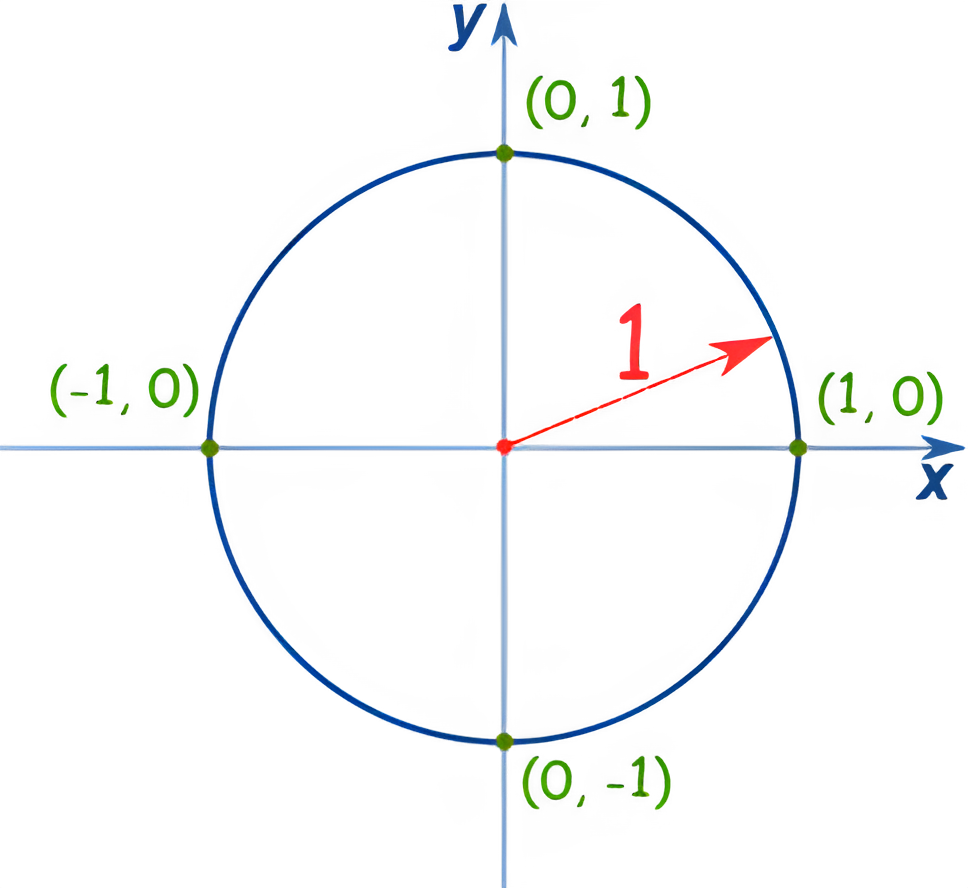
\includegraphics[width=0.8\textwidth]{unit-circle.png}
        \captionof{figure}{Unit Circle}
    \end{minipage}
    \begin{minipage}{0.5\textwidth}
        \centering
        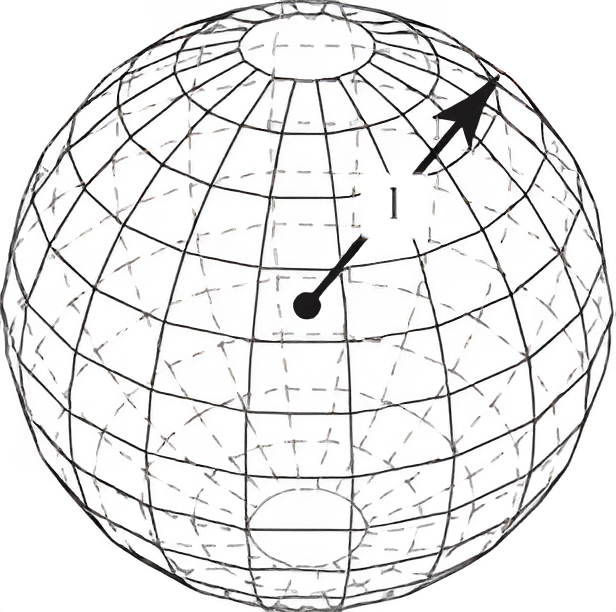
\includegraphics[width=0.8\textwidth]{unit-sphere.png}
        \captionof{figure}{Unit Sphere}
    \end{minipage}
\end{illustrationbox}

\begin{examplebox}
    The equation of a sphere centered at \( (2,2,1) \) with radius \( r = 3 \) is:
    \[
        (x - 2)^2 + (y - 2)^2 + (z - 1)^2 = 9
    \]
\end{examplebox}

\begin{examplebox}
    The equation of a sphere centered at \( (-1,0,-4) \) with radius \( r = \sqrt{5} \) is:
    \[
        (x + 1)^2 + y^2 + (z + 4)^2 = 5
    \]
\end{examplebox}

\begin{exercisebox}
    Given the equation:
    \[
        x^2 + y^2 + z^2 - 2x - 4y + 8z + 17 = 0
    \]
    Find the center and radius of the sphere.
\end{exercisebox}

\subsubsection*{Describing the Region Between Two Spheres}
\addcontentsline{toc}{subsubsection}{Describing the Region Between Two Spheres}

\begin{examplebox}
    Describe the following region in 3D space:
    \[
        2 \leq x^2 + y^2 + z^2 < 5
    \]

    \begin{solutionbox}
        Consider the two spheres:
        \begin{itemize}
            \item Sphere 1: \( x^2 + y^2 + z^2 = 5 \)
            \item Sphere 2: \( x^2 + y^2 + z^2 = 2 \)
        \end{itemize}

        The region is the set of points that lie inside the sphere of radius \( \sqrt{5} \) (exclusive) and outside the sphere of radius \( \sqrt{2} \) (inclusive).

        \begin{center}
            \begin{minipage}{0.3\textwidth}
                \centering
                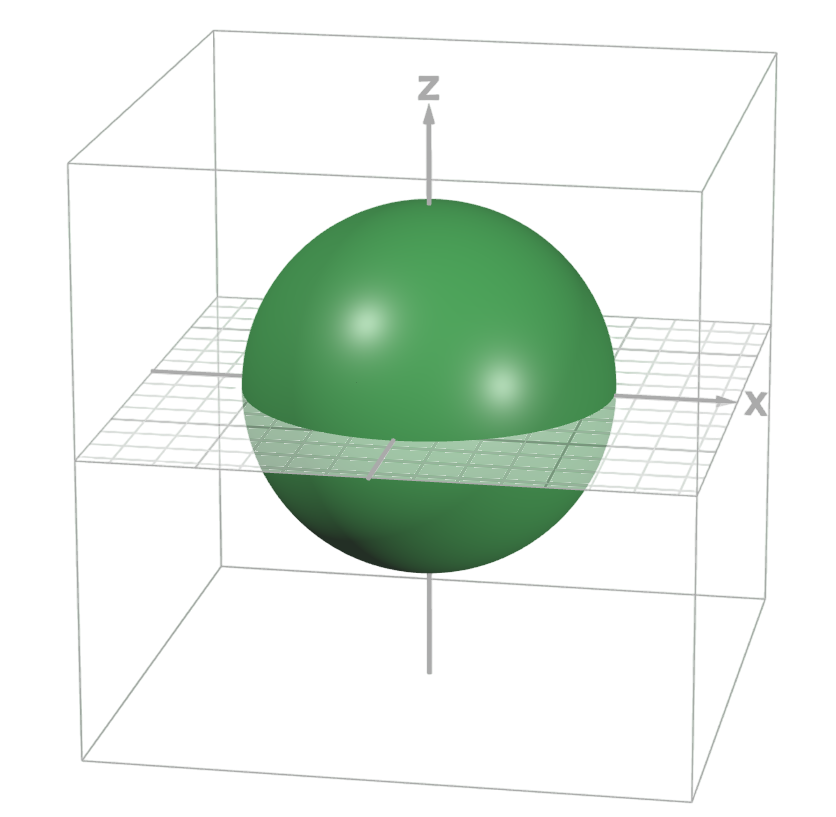
\includegraphics[width=0.9\textwidth]{region between 2.png}
                \captionsetup{justification=centerlast}
                \captionof{figure}{Region Between Spheres}
            \end{minipage}%
            \hfill
            \begin{minipage}{0.3\textwidth}
                \centering
                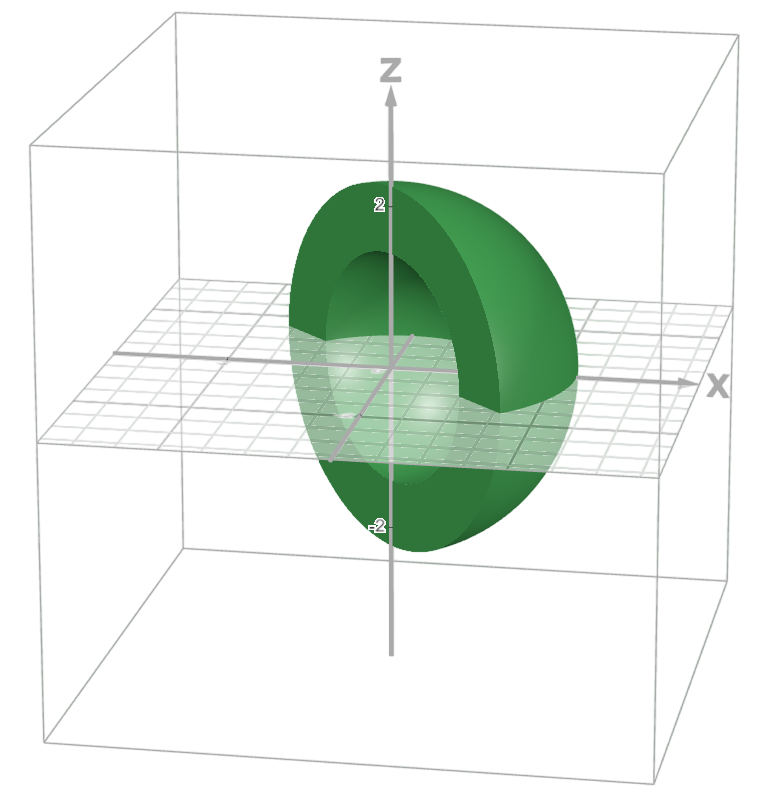
\includegraphics[width=0.9\textwidth]{region between 2 see thru.png}
                \captionsetup{justification=centerlast}
                \captionof{figure}{Region Between Spheres (Cut)}
            \end{minipage}%
            \hfill
            \begin{minipage}{0.3\textwidth}
                \centering
                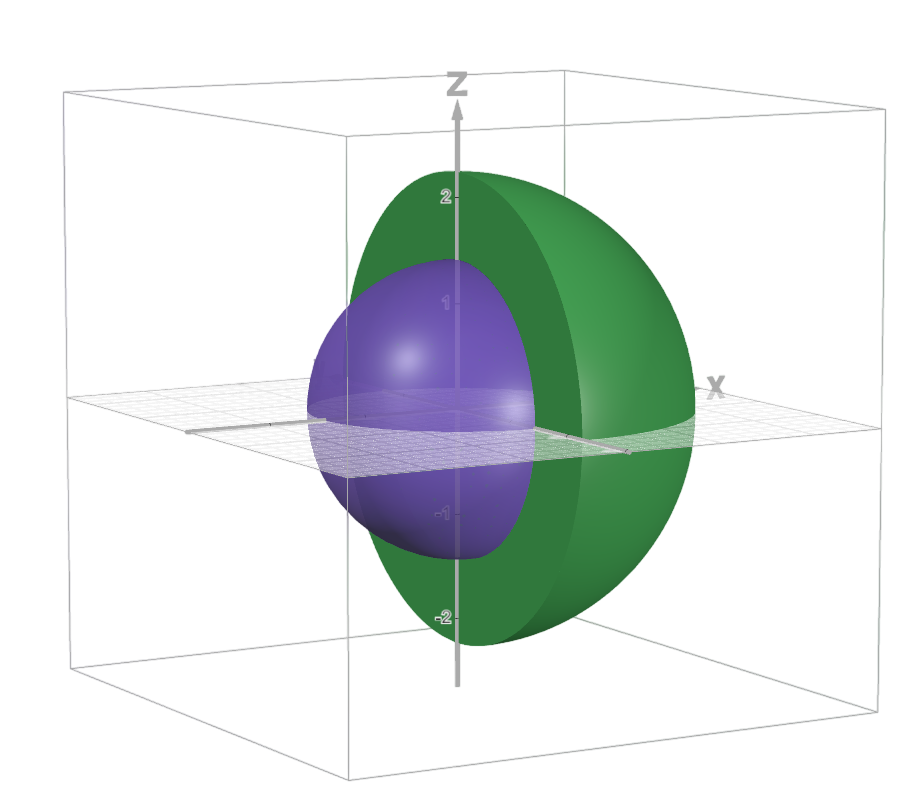
\includegraphics[width=0.9\textwidth]{region between 2 see thru with inner sphere.png}
                \captionsetup{justification=centerlast}
                \captionof{figure}{Region Between Spheres (Inner Sphere)}
            \end{minipage}
        \end{center}        
    \end{solutionbox}
\end{examplebox}

\subsection*{Introduction to Vectors}
\addcontentsline{toc}{subsection}{Introduction to Vectors}

A \textbf{vector} is a quantity that has both magnitude and direction. It is represented by an arrow, with the length of the arrow representing the magnitude and the direction of the arrow representing the direction.

\begin{notebox}
A vector can additionally be denoted by its \textbf{initial} and \textbf{terminal} points. The \textbf{position vector} of a point \( P \) is the vector that starts at the origin and ends at \( P \).
\end{notebox}

\begin{examplebox}
    Find the vector starting from point \( A(-1,3) \) and ending at point \( B(2,-1) \).
    \begin{solutionbox}
        The vector is given by:
        \[
            \vv{u} = \vv{AB} = B - A = \langle 2 - (-1), -1 - 3 \rangle = \langle 3, -4 \rangle
        \]
    \end{solutionbox}
\end{examplebox}
\begin{tipbox}
    There are two takeaways:
    \begin{itemize}
        \item Vectors have a length;
        \item Vectors have a direction.
    \end{itemize}
\end{tipbox}

\subsubsection*{Equivalent Vectors}
\addcontentsline{toc}{subsubsection}{Equivalent Vectors}

\begin{definitionbox}
    Two vectors are \textbf{equivalent} if they have the same magnitude and direction, regardless of their initial points.
\end{definitionbox}

\end{document}
